\documentclass[a4paper,openright,11pt]{article}
\date{}
\usepackage[spanish]{babel}
\usepackage{graphicx}
\usepackage{amssymb}
\usepackage{fancyhdr}
\usepackage{multirow}
\usepackage[utf8]{inputenc}
\usepackage{fancyhdr}
\usepackage{float}
\usepackage{color}
\usepackage{listings}

\begin{document}
\include{glosarioacronimos}
\renewcommand{\tablename}{Tabla}
\renewcommand{\listtablename}{\'Indice de tablas}
\renewcommand{\headrulewidth}{0.3pt}
\renewcommand{\footrulewidth}{0.3pt}
\newpage

\begin{titlepage}
	\begin{center}
		\vspace*{-1in}
		\begin{figure}[htb]
			\begin{center}
				
\includegraphics[width=10cm]{ug}
			\end{center}
		\end{figure}
		\vspace*{0.1in}
		\begin{Large}
			Ingeniería en Sistemas, Informática y \\Ciencias de la Computación\\
		\end{Large}
		\vspace*{0.2in}
		\begin{Large}
			Seminario Profesional II\\
		\end{Large}
		\vspace*{0.9in}
		\begin{LARGE}
			\textbf{\LARGE MAYALENG} \\
			\begin{figure}[htb]
				\begin{center}
					
\includegraphics[width=4cm]{ml}
				\end{center}
			\end{figure}
		\end{LARGE}
		\vspace*{0.9in}
		\begin{large}
			Autores:\\
			Douglas Figueroa \\
			Alexander Baquiax
		\end{large}
		\vspace*{0.3in}
		\\
		\rule{90mm}{0.1mm}\\
		\begin{large}
			Supervisado por: \\
			Ing. Jack Trachtenberg \\
			Ing. Axel Benavides
		\end{large}
	\end{center}
\end{titlepage}
\newpage

\tableofcontents

\cleardoublepage
\listoffigures

\cleardoublepage
\listoftables

\newpage

\pagestyle{fancy}
\rfoot{
\includegraphics[width=.08\textwidth]{ml}}
\lfoot{MayaLeng}
\section{Introducción}
Mayaleng más que una aplicación es un algoritmo con la capacidad de recibir un input, en nuestro caso, una palabra, una frase, un párrafo, una cantidad de texto muy grande, en español y retornar un output, (el texto de entrada), en una lengua maya. \\

Una herramienta de traducción y para conocimiento de la cultura de Guatemala.\\

La cultura en Guatemala es muy grande, uno de los propósitos de este proyecto es poder aportar a expandir el conocimiento en las lenguas mayas, una rama que forma gran parte de la cultura, por medio de un algoritmo de traducción, utilizando diferentes tecnologías, hacemos dicho aporte, creando un traductor de español e inglés a una lengua maya, el Kaqchikel.\\

Una aplicación móvil y web nos ayudará a expandir el conocimiento de esta lengua maya, la tecnología cada vez es más accesible, los teléfonos inteligentes y las computadores cada vez son más comunes en los hogares, lo que nos ayuda a deducir que el alcance puede ser mayor. Pero no solamente estamos enfocando esta herramienta al uso particular de personas, también se enfoca a que sea una herramienta de trabajo para quienes enseñan a otros el español, en este caso es un profesor quien utiliza la herramienta y es cierto que esta persona ya conoce la lengua maya pero con la herramienta puede generar su propia documentación para los alumnos que este tenga.\\

Utilizamos muchas herramientas para la construcción de este proyecto, MySQL, LiguaKit, PHP, Symfony, Ionic, API's; herramientas de las cuales iremos hablando en el desarrollo del proyecto.
\newpage

\section{Objetivos}
\subsection{Objetivo General}
Crear una herramienta de traducción de la lengua maya Kaqchikel.
\subsection{Objetivos Espec\'ificos}
\begin{itemize}
    \item Crear una aplicación\'on móvil (Android y iOS) para traducción del Kaqchikel.
    \item Dar a conocer la cultura de nuestro pa\'is Guatemala.
    \item Brindar la capacidad a profesores y personas en general de traducir documentos para facilitar su trabajo en los lugares d\'onde imparten clases dentro de nuestro pa\'is y los cuales no dominan el español.
\end{itemize}
\newpage

\section{El Problema}
\subsection{¿Cuál es el problema?}
El problema analizado para querer desarrollar esta herramienta fue desde un punto de vista cultural, ya que en Guatemala existen muchas lenguas mayas, de las cuales pocas personas en el pa\'is dominan como mínimo una. Estas forman parte de nuestro patrimonio cultural. Alrededor del mundo Guatemala es conocida por los puntos turísticos con los que contamos, regularmente estos se encuentran en los departamentos donde al menos existe una lengua Maya.  Como guatemaltecos deberíamos de poder comunicarnos con la gente de nuestro pa\'is, ya que en algunos departamentos no se habla mucho en español sino que hablan en una lengua maya, sin embargo ese no es el caso. No hemos encontrado tantas herramientas claras que nos faciliten dicha tarea, queremos ser de los primeros en brindar dicha herramienta.\\

En este momento sugerimos Kaqchikel, la forma en que solucionamos el problema de la comunicación es teniendo una aplicación m\'ovil la cu\'al hará una traducción en nuestro idioma natal a Kaqchikel, sencillamente quien utilice la aplicación deberá ingresar el texto y en una casilla aparte aparecer\'a la traducci\'on del texto, algo similar a google translate.\\

Le ahorraremos al usuario tener que escribir algunas de las frases o palabras m\'as utilizadas, ya que tendremos una secci\'on donde diremos como se dicen esas frases, cosas b\'asicas como saludar, despedirse, hasta algo m\'as formal, un ejemplo ser\'ia preguntar d\'onde se encuentra el baño, preguntar el nombre de una persona y frases similares.\\
\newpage

\section{Estudio de Factibilidad}
\subsection{Factibilidad Funcional}
\subsubsection{Resultados de Encuesta}
\begin{figure}[H]
	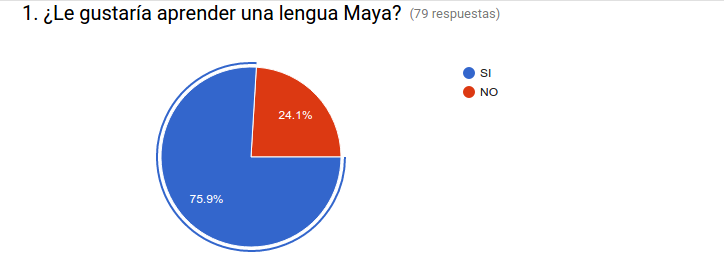
\includegraphics[width=1.0\textwidth]{e1}
	\caption{Aprender una lengua maya}
	\label{fig:e1}
	Del total de personas que contestaron la encuesta podemos observar que más del 75\% de las personas está interesada en aprender una lengua maya. Con esto conocemos las personas que darían uso a la aplicación de traducción al momento de tenerla.
\end{figure}
\begin{figure}[H]
	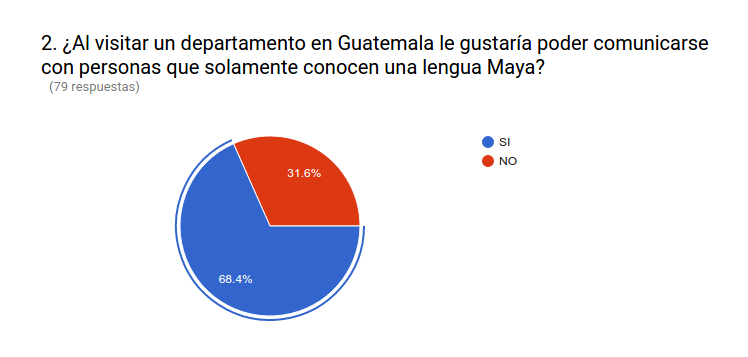
\includegraphics[width=1.0\textwidth]{e2}
	\caption{Comunicación en lengua maya}
	\label{fig:e2}
	En la gráfica podemos observar que casi la tercera parte de las personas les gustaría entablar una conversación en una lengua maya, estas personas pueden estar enlazadas a la pregunta 1, que contestaron con un sí.
\end{figure}
\begin{figure}
	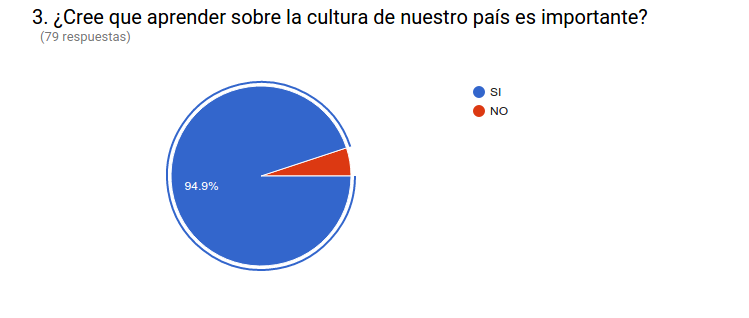
\includegraphics[width=1.0\textwidth]{e3}
	\caption{Cultura importante}
	\label{fig:e3}
	En esta pregunta vemos que casi todos contestaron que sí, hay un pequeño porcentaje que piensa que la cultura de nuestro país no es algo importante.
\end{figure}
\begin{figure}
	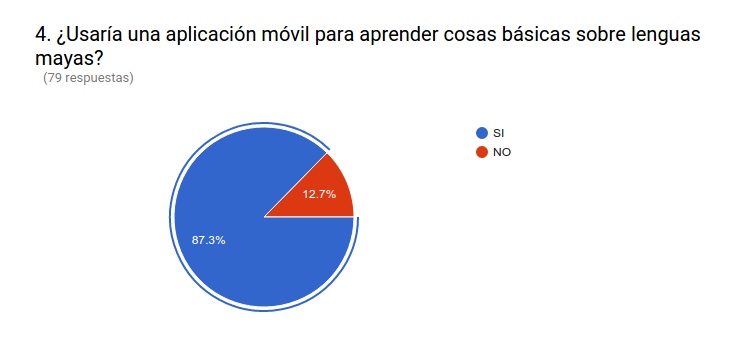
\includegraphics[width=1.0\textwidth]{e4}
	\caption{Una aplicación móvil}
	\label{fig:e4}
	Todas las personas que entrevistamos cuentan con un teléfono inteligente, de todas esas personas la mayoría está dispuesta a instalar y utilizar nuestra aplicación en su teléfono.
\end{figure}
\begin{figure}
	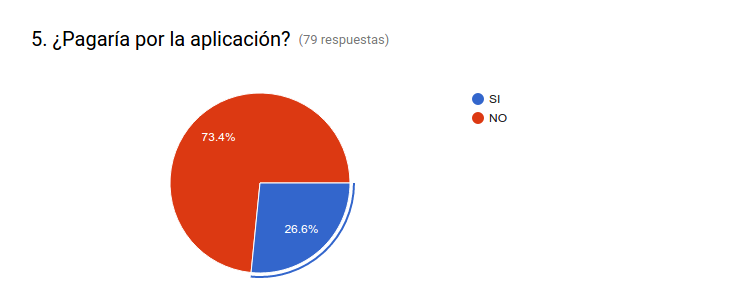
\includegraphics[width=1.0\textwidth]{e5}
	\caption{Pago por la aplicación}
	\label{fig:e5}
	En esta pregunta creímos que el 100\% de las personas contestaría con un no, sin embargo un pequeño porcentaje de personas estaría dispuesta a pagar por la aplicación.
\end{figure}
\begin{figure}
	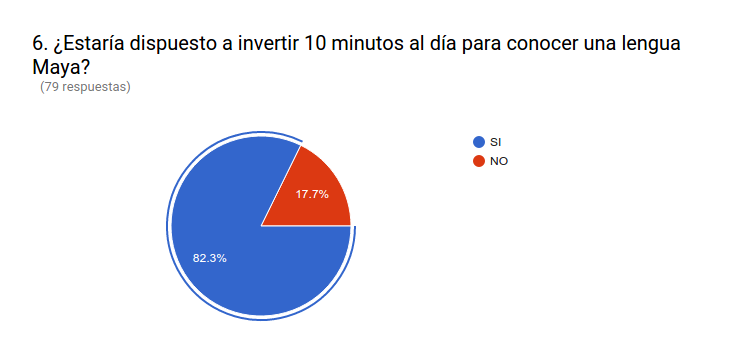
\includegraphics[width=1.0\textwidth]{e6}
	\caption{Inversión de tiempo}
	\label{fig:e6}
	Diez minutos es un tiempo pequeño para revisar una aplicación móvil, tiempo que la mayoría de los entrevistados estaría dispuesto a utilizar para revisar el traductor maya.
\end{figure}

\subsubsection{Tablas Comparativas}
\begin{table}[H]
	\resizebox*{14cm}{!}{
	\begin{tabular}{|r|c|c|c|c|}
	\hline
	Funcionalidad & Google Translate & Glosbe.com & Profesor & MayaLeng\\
	\hline
	Traducci\'on de palabras & \checkmark & \checkmark & \checkmark & \checkmark\\
	\hline
	Traducci\'on	 bidireccional & \checkmark & x & \checkmark & x\\
	\hline
	Traducci\'on de frases  & \checkmark & x & \checkmark & \checkmark\\
	\hline
	Traducci\'on precisa & \checkmark & x & \checkmark & \checkmark\\
	\hline
	Herramienta de traducci\'on de documentos & \checkmark & x & \checkmark & \checkmark\\
	\hline
	\end{tabular}}
\caption{Comparativa de Funcionalidades}
	A nivel de funcionalidad nuestro competidor más grande es un profesor, quién posee las habilidades necesarias para desempeñar el trabajo de traductor, sin embargo hablamos de una persona contra una herramienta de tecnología que es más factible.
\end{table}

\begin{table}[H]
	\resizebox*{14cm}{!}{
	\begin{tabular}{|r|c|c|c|c|}
	\hline
	Caracter\'istica & Google Translate & Glosbe.com & Profesor & MayaLeng\\
	\hline
	Descripci\'on de palabras & x & \checkmark & \checkmark & x\\
	\hline
	Intuitivo & \checkmark & x & \checkmark & \checkmark\\
	\hline
	Es gratis  & \checkmark & \checkmark & x & \checkmark\\
	\hline
	Siempre disponible & \checkmark & \checkmark & x & \checkmark\\
	\hline
	F\'acil de obtener/contactar & \checkmark & \checkmark & x & \checkmark\\
	\hline
	\end{tabular}}
\caption{Comparativa de Caracter\'isticas}
Cuando evaluamos características la tecnología toma el control en aportar más cosas factibles que un profesor (nuestra mayor competencia), y podemos observar que MayaLeng cumple con casi todas las características de la evaluación realizada.
\end{table}

\subsubsection{Conclusión}
Nuestra herramienta cumple con ser una herramienta factible, en base a las encuestas, conocemos la opinión de las personas y vemos que comportamiento tendrían si tuvieses la herramienta en sus manos, con las tablas comparativas pudimos ver a que nivel nos encontramos comparándonos con otras soluciones similares.

\newpage
\subsection{Factibilidad T\'ecnica}
Pretendemos aprovechar el apogeo de los m\'oviles y tratar de crear una buena oportunidad para introducir nuestro proyecto.\\
Actualmente existen dos grandes sistemas operativos que domina la industria de los m\'oviles:. iOS y Android. Estamos conscientes de que desarrollar de forma nativa para ambas plataformas nos representar\'ia un poco m\'as de tiempo, que implicar\'ia restarle tiempo a la parte que en verdad es importante. Por lo cual usaremos IONIC, framework que nos permite desarrollar de manera sencilla aplicaciones m\'oviles usando las tendencias de Responsive Web Design. \\

Lo interesante de este proyecto no radica en la aplicaci\'on m\'ovil, de hecho la aplicaci\'on s\'olo ser\'a una forma de consumir nuestro verdadero sistema.\\

La idea de este proyecto radica en hacer un compilador que pueda usar una gram\'atica y una fuente de palabras de esa gram\'atica, y traducir de ellas las palabras al español. En pocas palabras nuestro proyecto radica en hacer un compilador de idiomas mayas.\\

Durante el transcurso de nuestra carrera ya hicimos un compilador, con todas las fases b\'asicas que uno de ellos debe tener. Ahora nos pusimos el reto de hacer un compilador gen\'erico. Para esta primera versi\'on usaremos dos idiomas Mayas.\\

Creemos tener los conocimientos necesarios para la construcci\'on de esto. Uno de los inconvenientes m\'as grandes era que ninguno de los dos sabemos hablar un idioma Maya, pero nos apoyamos en la documentaci\'on que distintas personas a lo largo de la historia han construido.\\ 

La idea es construir un API al que se le pueda dar como input un texto, p\'arrafo, documento y que la salida sea otro documento pero con texto traducido. Ahora tenemos una base de datos con 15 mil palabras aproximadamente del Kaqchikel. La DB esta montada en un DBMS MySQL. El API fue construido en Symfony2. El core de traducci\'on fue realizado con LinguaKit.

\subsubsection{Conclusión}
La tecnología utilizada cubre con las necesidades para el proyecto, nos ayuda a que las tareas sean optimizadas, utilizando menos recursos y optimización de tiempo, lo cuál es un punto muy importante a considerar.

\subsection{Factibilidad Econ\'omica}
Bas\'andonos en nuestra calendarizaci\'on de tareas para el desarrollo del proyecto, hemos estimado los siguientes costos para el desarrollo de la aplicaci\'on, los gastos son a nivel de costo de servidor, por compra del dominio, licencias para subir aplicaci\'on y gastos en papel, en impresi\'on del manual de usuario.\\

\begin{table}[h]
	\resizebox*{15cm}{!}{
	\begin{tabular}{|l|r|r|}
	\hline
	\textbf{Servicios} &  & \textbf{Precio(\$.) al mes}\\
	\hline
	Amazon EC2 & \$0.013 por hora. & 9.36\\
	\hline
	Google API & \$20 por 1 million de caracteres. & 20.00\\
	\hline
	 & \textbf{Total} & \textbf{29.36}\\
	\hline
	\textbf{Desarrollador (\$20/hora)} & \textbf{Horas} & \textbf{Precio (\$)}\\
	\hline
	Configuración de servidores & 2 & 40.00\\
	\hline
	Configuracion de Symfony y LinguaKit & 8 & 120.00\\
	\hline
	Migración de diccionario en excel a  DB & 4 & 80.00\\
	\hline
	Información a palabras usando RAE & 4 & 80.00\\
	\hline
	Desarrollo de Bundle para traducción & 4 & 80.00\\
	\hline
	Desarrollo de módulo para integrar ML Bundle con Linguakit. & 4 & 80.00\\
	\hline
	Aprendizaje de IONIC & 3 & 60.00\\
	\hline
	Inicio de comunicación al modulo de traducción & 5 & 100.00\\
	\hline
	Integración con Google Translate & 5 & 100.00\\
	\hline
	Documentación técnica & 20 & 400.00\\
	\hline
	Traducción de sitios web & 10 & 200.00\\
	\hline
	Traducción inversa Kaqchikel - Cualquier idioma & 6 & 120.00\\
	\hline
	Aplicación de grámatica Kaqchikel & 24 & 480.00\\
	\hline
	Traducción Kaqchikel -> Cualquier idioma & 10 & 200.00\\
	\hline
	\textbf{Total} & \textbf{109} & \textbf{2,140.00}\\
	\hline
	\hline
	\hline
	 & \textbf{Totales(\$)} & \textbf{Totales(Q)}\\
	\hline
	 & \textbf{2,169.36} & \textbf{16,270.20}\\
	 \hline
	\end{tabular}}
\caption{Factibilidad Econ\'omica}
\end{table}

\subsubsection{Conclusión}
Damos detalle de los gastos involucrados en este proyecto, el gasto de los servicios que adquirimos y el precio de realizar el proyecto tomado en horas, tenemos un total de 109 horas trabajadas con un costo de \$20 por hora, cantidad que mostramos al final en quetzales(Q.).
\newpage

\section{Kaqchikel}
\subsection{Lengua Maya Kaqchikel}
El idioma kaqchikel forma parte de los idiomas de Mesoamérica provenientes del tronco protomaya, de la rama lingüística K’iche’ y del tronco K’iche’ propio, donde comparte raíces con los idiomas K’iche’, Tz’utujil, Sakapulteko y Sipakapense. Según los especialistas es una de las lenguas que conservan mayor pureza del Periodo Clásico Maya después de las transformaciones del 900 d.C. Con un total de hablantes aproximadamente de medio millón de habitantes, más hablado en los siguientes departamentos:
\begin{itemize}
	\item Guatemala: Chuarrancho, San Juan Sacatepéquez, San Pedro Ayampuc, San Pedro Sacatepéquez y San Raymundo.
	\item Sacatepéquez: Magdalena Milpas Altas, San Antonio Aguas Calientes, Santa Catarina Barahona, San Lucas Sacatepéquez, San Bartolomé Milpas Altas, Santiago Sacatepéquez, Sumpango, Santa María de Jesús, Santo Domingo Xenacoj, San Miguel Dueñas, San Juan Alotenango y Santa Lucía Milpas Altas.
	\item Escuintla: Santa Lucía Cotzumalguapa.
	\item Sololá: Sololá, Panajachel, San Andrés Semetabaj, San Antonio Palopó, San José Chacayá, Santa Catarina Palopó, Santa Cruz La Laguna, Concepción y San Marcos La Laguna.
	\item Suchitepéquez: San Antonio Suchitepéquez, San Juan Bautista y Patulul.
	\item Baja Verapaz: parte del municipio de El Chol.
\end{itemize}
Esta área geográfica no ha variado en forma significativa desde el siglo XVI. El kaqchikel  forma parte de la identidad y de los valores culturales y sociales de la región, es un idioma auténtico ya que posee gramática y escritura y es una práctica de derecho lingüístico individual para resguardarlo, estudiarlo y enseñarlo en las escuelas. Constituye junto a las regiones mam y tz’utujil una de las regiones de mayor riqueza lingüística y social en Guatemala. \\

La comunidad lingüística kaqchikel se organiza alrededor de la familia y de las organizaciones sociales como la cofradía y las alcaldías indígenas, la tierra es sagrada y en donde el maíz y el frijol siguen siendo el punto medular de su alimentación. Fuerte como una Ceiba la comunidad kaqchikel brilla como el Corazón del Cielo y el Corazón de la Tierra.\\ 

\newpage
\subsection{Gramática}
Como se mencionaba el Kaqchikel es un idioma auténtico que posee su gramática, a continuación damos mención a parte de esa gramática.\\

\subsubsection{Alfabeto}
El alfabeto kaqchikel está conformado de los siguientes símbolos:\\
a - ä - b' - ch - ch' - e - ë - i - ï - j - k - l - m - n - o - ö - p - q - q' - r - s - t - t' - tz - tz' - u - ü - w - x - y - '

\subsubsection{Sustantivos}
Para los pronombres y sustantivos tenemos las siguientes reglas, hay prefijos que se anteponen dependiendo si el sustantivo empieza con una vocal o con una consonante:
\begin{table}[H]
\resizebox*{14cm}{!}{
	\begin{tabular}{|l|l|l|l|}
		\hline
		\textbf{Ante constante} & \textbf{Ante vocal} & \textbf{Clasificación} & \textbf{Ejemplo}\\
		\hline
		nu- & w- & 1a. Persona singular (yo) & nuch’atal - mi mesa\\
		\hline
		a- & aw- & 2a. Persona singular (tu) & ach’atal - tu mesa\\
		\hline
		ru-  & r- & 3a. Persona singular (él/ella) & ruch’atal - su mesa\\
		\hline
		qa- & q- & 1a. Persona singular (nosotros) & qawän - nuestra milpa\\
		\hline
		i- & iw- & 2a. Persona singular (ustedes) & iwawän - su milpa\\
		\hline
		ki- & k- & 3a. Persona singular (ellos/ellas) & kawän - sus milpas\\
		\hline
	\end{tabular}}
	\caption{Reglas gramaticales de Sustantivos}
\end{table}

\subsubsection{Plural}
Para aplicar la regla gramatical al uso de plurales no hay un uso en específico:
\begin{table}[H]
	\begin{center}
	\resizebox*{6cm}{!}{
		\begin{tabular}{|l|l|}
			\hline
			\textbf{Regla} & \textbf{Ejemplo}\\
			\hline
			Terminación: i’ & Patios - ruwa jayi'\\
			\hline
			Terminación: a’ & Perros - tz'i'a'\\
			\hline
		\end{tabular}}
	\end{center}
	\caption{Reglas gramaticales de Plurales}
\end{table}

\newpage
\subsubsection{Oraciones}
En la estructura de una oración en kaqchikel tenemos primero el predicado seguido del sujeto, resaltamos el predicado con negrita:
\begin{table}[H]
	\begin{center}
	\resizebox*{9cm}{!}{
		\begin{tabular}{|l|l|}
			\hline
			\textbf{Español} & \textbf{Kaqchikel}\\
			\hline
			Llegó el señor & \textbf{Xapon} ri achi\\
			\hline
			Los niños están muy cansados & \textbf{Yalan e kosinäq} ri ak'wala'\\
			\hline
		\end{tabular}}
	\end{center}
	\caption{Regla gramatical de una oración simple}
\end{table}
\newpage

\section{Marco Teórico}
\subsection{Lenguas Mayas}
En Guatemala contamos actualmente con más de 20 lenguas mayas,  los Acuerdos de Paz firmados en diciembre de 1996 hacen un compromiso de estado, el reconocimiento de los diferentes idiomas del país, lo cual hace que el país sea reconocido como uno multilingüe, y se hace constar en la Constitución que los idiomas mayas deberán respetarse y difundirse. Se han hecho esfuerzos, sin embargo los pocos habitantes que quedan hacen difícil la tarea. Muchos jóvenes de las nuevas generaciones no llegan a aprender el idioma indígena de sus padres. Actualmente los idiomas de mayor habla son el Kekchí, el Quiché, el Kaqchikel, el Mam y el Tzutujil, los cuales tienen algunos vocablos y reglas gramaticales en común. \\

Las lenguas mayenses derivan del protomaya, una protolengua (reconstrucción probable de la lengua origen de un grupo de lenguas), que pudo haberse hablado hace unos 5000 años a juzgar por el grado de diversificación interna en una región cercana a donde actualmente se hablan lenguas mayenses.

\begin{figure}[H]
	\centering
	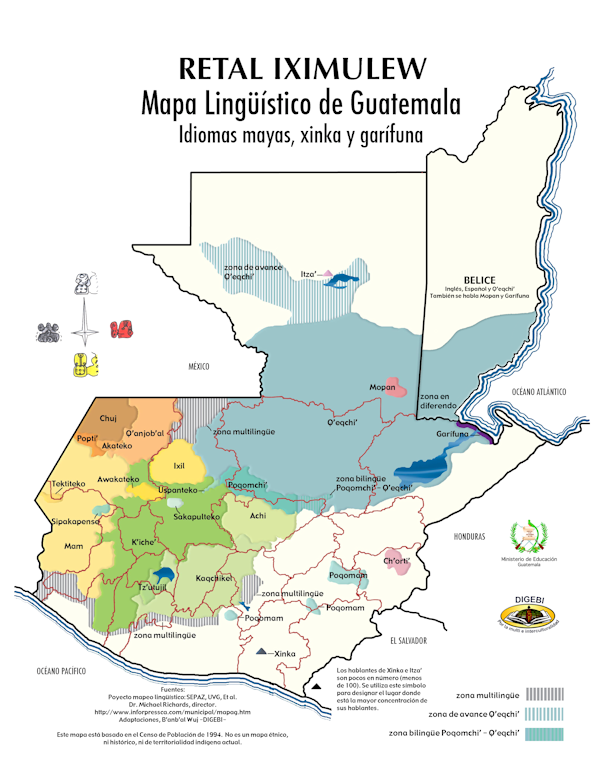
\includegraphics[width=0.55\textwidth]{mapa}
	\caption{Mapa de lenguas mayas}
	\label{fig:map}
\end{figure}
En este mapa se puede observar como están distribuidas las lenguas mayas alrededor del país.

\begin{figure}[H]
	\centering
	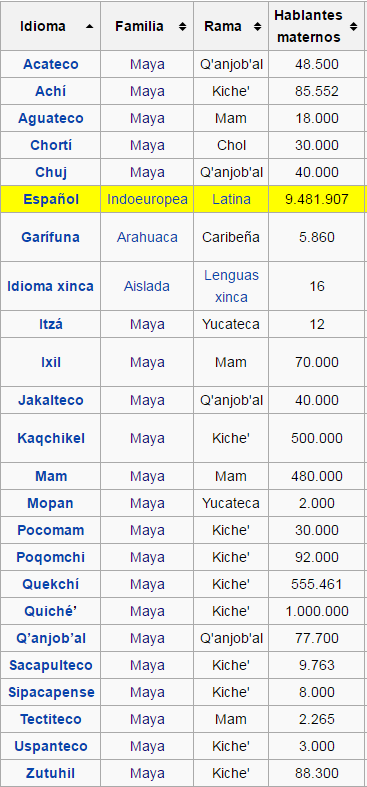
\includegraphics[width=0.6\textwidth]{tablalenguas}
	\caption{Tabla de lenguas mayas}
	\label{fig:tabla}
\end{figure}
En esta tabla tenemos a detalle la cantidad de hablantes de cada una de las lenguas habladas en el país, de las cuales la predominante es el español, siendo casi los 9,500 millones de habitantes, siendo Quiché' la segunda más hablada, en tercer y cuarto lugar el Quekchí y Kaqchikel respectivamente, con medio millón de hablantes.

\begin{figure}[H]
	\centering
	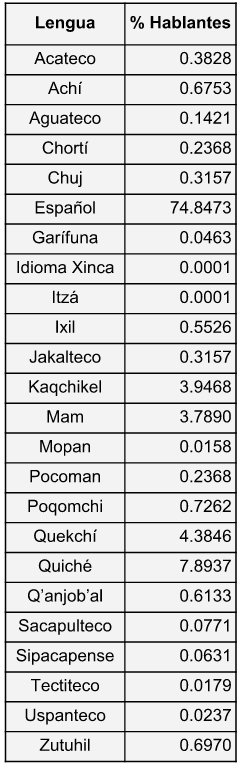
\includegraphics[width=0.3\textwidth]{porhablantes}
	\caption{Porcentaje de hablantes de lenguas mayas}
	\label{fig:porc}
\end{figure}
De la tabla anterior, porcentualmente las lenguas más habladas en el país son el español, con un 74.85\%, Quiché con 7.89\%, y Quekchí y Kaqchikel con 4.38\% y 3.95\% respectivamente.

\newpage
\subsection{Tecnologías Involucradas}
Como parte de las herramientas involucradas para el desarrollo de este proyecto tenemos:
\begin{table}[H]
	\begin{center}
	\resizebox*{5cm}{!}{
		\begin{tabular}{|l|l|}
			\hline
			1. & MySQL\\
			\hline
			2. & PHP\\
			\hline
			3. & RAE\\
			\hline
			4. & LinguaKit\\
			\hline
			5. & Symfony\\
			\hline
			6. & Ionic\\
			\hline
			7. & Formularios de Google\\
			\hline
			8. & LaTex\\
			\hline
			9. & Wordpress\\
			\hline
			10. & Google API\\
			\hline
		\end{tabular}}
	\end{center}
	\caption{Tecnologías Involucradas}
\end{table}
A continuación hablaremos un poco acerca de cada una.

\subsubsection{MySQL}
Es un sistema de gestión de bases de datos relacional desarrollado bajo licencia dual GPL/Licencia comercial por Oracle Corporation y está considerada como la base datos open source más popular del mundo, fue desarrollada inicialmente por MySQL AB, una empresa que era muy conocida por ser de las más grandes empersas de software libre del mundo. Fue adquirida por Sun Microsystems en el 2008, y luego ésta fue comprada por Oracle Corporation en el 2010. La base de datos se distribuye en varias versiones, una Community, distribuida bajo la Licencia pública general de GNU, versión 2, y varias versiones Enterprise, para aquellas empresas que quieran incorporarlo en productos privativos. En su mayor parte está desarrollada en ANSI C y C++.MySQL es muy utilizado en aplicaciones web.

\subsubsection{PHP}
Es común que trabaje en conjunto con MySQL; es un lenguaje del lado del servidor y una herramienta muy poderosa para hacer páginas web dinámicas e interactivas, es un lenguaje de código abierto ampliamente utilizado. Corre en sistemas muy grandes como lo son WordPress y Facebook. Se puede crear, abrir, leer, escribir, borrar y cerrar archivos en el servidor, recopilar datos de formularios, enviar y recibir cookies. Con PHP se puede ejecutar funciones CRUD en la base de datos, podemos tener un control de sesiones por usuario y cifrado de datos.

\subsubsection{RAE}
Es una institución cultural que se dedica a la regularización lingüística mediante la promulgación de normativas dirigidas a fomentar la unidad idiomática entre o dentro de los diversos territorios que componen el llamado mundo hispanohablante. Fue fundada en 1713 por iniciativa de  Juan Manuel Fernández Pacheco, VIII marqués de Villena y duque de Escalona.

\subsubsection{LinguaKit}
Es una herramienta con la cual explorar, analizar y obtener una mejor información de textos y documentos escritos, posee un resumidor, un analizador de sentimiento y un extractor de las palabras clave que dan sentido a un texto, está pensado para que toda persona que posea interés lingüístico pueda sacarle el máximo provecho a los textos escritos. Linguakit hace un análisis completo del texto que se le mande, puede conocer el número de palabras y frases del texto, y su tipología, un resumen de su contenido así como el sentimiento de ese resumen. Además, las entidades más importantes que allí se mencionan, las palabras más frecuentes y el contexto en el que aparece la palabra clave escogida.

\subsubsection{Symfony}
Es un framework conjunto de componente PHP, un marco de aplicaciones web  diseñado para optimizar el desarrollo de las aplicaciones web basado en el patrón Modelo Vista Controlador. Symfony está desarrollado completamente en PHP 5.3. Ha sido probado en numerosos proyectos reales y se utiliza en sitios web de comercio electrónico de primer nivel. Symfony es compatible con la mayoría de gestores de bases de datos, como MySQL, PostgreSQL, Oracle y Microsoft SQL Server. Se puede ejecutar tanto en plataformas *nix (Unix, Linux, etc.) como en plataformas Windows.

\subsubsection{IONIC}
Es una herramienta, gratuita y open source, para el desarrollo de aplicaciones híbridas basadas en HTML5, CSS y JS. Está construido con Sass y optimizado con AngularJS. Ionic está construido para ser rápido gracias a la mínima manipulación del DOM (interfaz de plataforma que proporciona un conjunto estándar de objetos para representar documentos HTML, XHTML y XML), con cero jQuery y con aceleraciones de transiciones por hardware. Utilizando Ionic se desarrolla una vez y se puede compilar para varias plataformas, posee un CLI muy potente en que con un sólo comando se puede crear, construir, probar y compilar las aplicaciones en cualquier plataforma.

\subsubsection{Formularios de Google}
Utilizamos los formularios de Google que es una herramienta para realizar encuestas y crearlas de forma rápida y tener actualizaciones inmediatas de lo que las personas están contestando, posee un formato de opciones para que el usuario pueda contestar, se pueden tener imágenes y videos de Youtube, genera gráficas por cada pregunta en tiempo real.

\subsubsection{\textbf{\LaTeX}}
Es un sistema de composición de textos, orientado a la creación de documentos escritos que presenten una alta calidad tipográfica. Por sus características y posibilidades, es usado de forma especialmente intensa en la generación de artículos y libros científicos que incluyen, entre otros elementos, expresiones matemáticas, está formado por un gran conjunto de macros de TeX, escrito por Leslie Lamport en 1984, con la intención de facilitar el uso del lenguaje de composición tipográfica. Es muy utilizado para la composición de artículos académicos, tesis y libros técnicos, dado que la calidad tipográfica de los documentos realizados es comparable a la de una editorial científica de primera línea. \LaTeX \hspace{0.1cm} es software libre bajo licencia LPPL.

\subsubsection{WordPress}
Es un software que se puede utilizar para crear fantásticas webs, blogs o aplicaciones. Es, al tiempo, gratis y de un precio incalculable. Dicho de forma sencilla, WordPress es el sistema que se utilizar como una herramienta de publicación muy buena y fácil de utilizar. WordPress es una herramienta que la crean y mantienen cientos de voluntarios de la comunidad, y hay miles de plugins y temas disponibles para transformar un sitio web en cualquier cosa que se pueda imaginar. Más de 60 millones de personas han elegido WordPress. Es muy famoso por que su instalación es fácil de realizar y en un corto tiempo, para ser exactos 5 minutos. Puede ser instalado en varios idiomas, puede ser actualizado después de ser instalado y contiene un conjunto de temas disponibles.

\subsubsection{Google API}
Es un set de servicios que Google ofrece. De este utilizamos el API de Google Translate. Lo utilizamos para realizar HTTP Request que puedan traducirnos de cualquier idioma soportado al español. Esto se debe a que nuestro módulo de traducción es Español - Kaqchikel.\\ 
Esto nos da una oportunidad de que alguien de habla anglosajona pueda de igual forma usar la aplicación sin necesidad de traducir su oración a Español.\\

Habíamos mencionado en la sección 3, \textbf{\textit{El Problema}}, que nuestra problemática era desde un punto cultural, un problema de comunicación interna por falta de conocimiento, porque no conocemos las lenguas mayas, no las podemos hablar, y tampoco encontramos información fácil sobre ellas, no es cómo hacer una traducción en Google translate y saber cómo se escribe alguna palabra que necesitamos usar, eso nos lleva al siguiente análisis. \\
\newpage

\section{MayaLeng}
\subsection{MayaLeng}
\subsubsection{¿En qué consiste?}
La solución planteada a esta problemática es la construcción de un algoritmo que nos ayude a establecer esta comunicación que no se posee, trabajamos en un traductor con el cual podamos transformar frases en español a frases en una lengua maya, como lengua inicial hemos escogido el Kaqchikel. Una vez construido el algoritmo de traducción necesitamos un dispositivo por el cual podamos darle uso a dicha herramienta, el dispositivo que elegimos para nuestra implementación es un teléfono inteligente, lo aplicamos para teléfonos que tengan instalado los sistemas operativos \textbf{Android} y \textbf{iOS}; Android es un sistema operativo móvil creado por Google Inc, y iOS es un sistema operativo móvil creado por Apple Inc.

El mercado de teléfonos inteligentes cada vez crece más, con la llegada del 4G el mercado móvil dio un nuevo paso y más personas tienen más fácil acceso al internet por medio de un dispositivo móvil, por lo que tener aplicaciones que requieran internet cada vez es menos costoso para el usuario, en el 2014 se estimó que había una cantidad de 21.7 millones de líneas telefónicas móvil en el país.

\subsubsection{¿Qué hicimos?}
Creamos una aplicación móvil con el nombre de \textbf{\textit{MayaLeng}} utilizando \textbf{ionic}, este es un framework que nos permite hacer un solo desarrollo y compilar nuestro programa una sola vez y generar una aplicación para iOS y Android; MayaLeng consume el algoritmo de traducción.

\subsubsection{¿Cómo funciona?}
Lo que se requiere para su funcionamiento es escribir una palabra, una frase, una oración o un párrafo en una caja de texto, una vez MayaLeng haya iniciado, este texto llega al algoritmo, contamos con un diccionario de español-kaqchikel, el diccionario lo llenamos con su respectivo tipo de palabra, el cual obtuvimos utilizando la \textbf{RAE}, una institución cultural dedicada a la regularización lingüística.\\
Utilizamos su API con un scritp desarrollado en \textbf{PHP} que es un lenguaje de programación que se ejecuta del lado del servidor, es considerado uno de los lenguajes más flexibles, potentes y de alto rendimiento,  con este script obtenemos el tipo de palabra (sustantivo, pronombre, verbo, etc.) de cada una de las contenidas en el diccionario.\\\\

El diccionario está almacenado en una base de datos \textbf{MySQL} que es sistema gestor de base de datos (DBMS) de licencia gratuita; mandamos nuestra oración a otra herramienta llamada \textbf{LinguaKit} que nos devuelve cada palabra de nuestra oración con su respectivo tipo de palabra. Las palabras podrían ser artículo, pronombre, verbos; una vez tenemos esos resultados los enlazamos con el tipo de palabra con el que ya contamos en la base de datos y ya teniendo la información, con \textbf{Symfony}, un framework diseñado para optimizar el desarrollo de las aplicaciones web basado en el patrón MVC (Modelo Vista Controlador), construímos la oración.\\\\

\subsubsection{¿Cómo construimos la oración?}
Para explicar la construcción mostramos la siguiente imagen:\\
\begin{figure}[H]
	\centering
	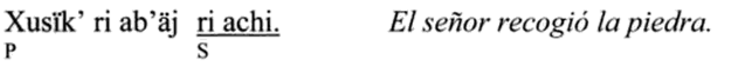
\includegraphics[width=0.9\textwidth]{oracion}
	\caption{Oración español-kaqchikel}
	\label{fig:kaq}
\end{figure}
La estructura de una oración simple en español es:
\begin{center}
	\textit{Sujeto - Predicado}\\
\end{center}

La estructura de una oración simple en Kaqchikel es:
\begin{center}
	\textit{Predicado - Sujeto}\\
\end{center}

Basándonos en la respuesta de \textit{Linguakit}, que nos devuelve que palabras forman parte del sujeto, y cuales del predicado, podemos colocar cada palabra en su orden correspondiente en base a la estructura de Kaqchikel que se obtuvo, este procedimiento lo realizamos para oraciones simples.

\newpage
\subsection{Diagrama Entidad-Relación}
\begin{figure}[H]
	\centering
	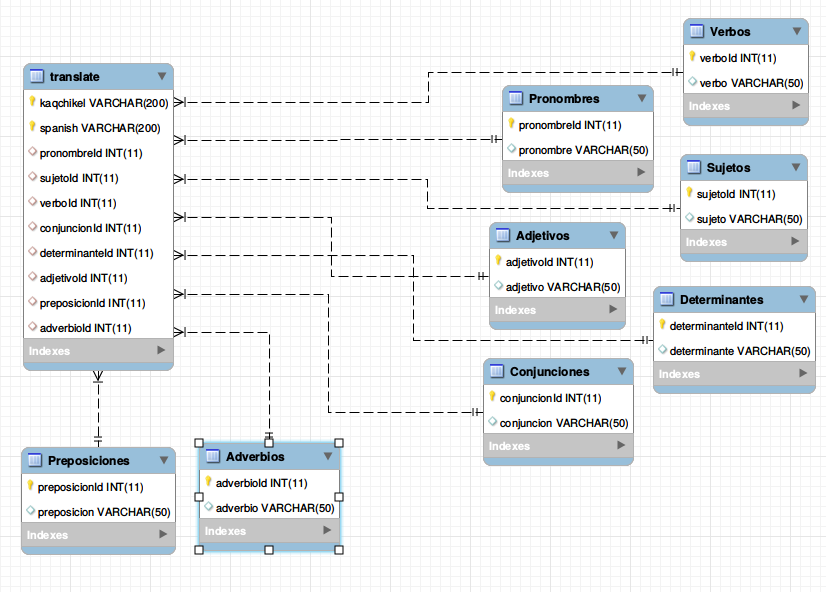
\includegraphics[width=0.9\textwidth]{er}
	\caption{Diagrama Entidad Relación}
	\label{fig:er}
\end{figure}
La base de datos está compuesta por una tabla principal que contiene el vocabulario, con la palabra en español y su traducción a Kaqchikel, una tabla con la estructura gramatical (sujeto, verbo, adjetivo, etc.), y una tercer tabla que nos servirá para enlazar nuestro vocabulario con el tipo de palabra a la que aplique (por ejemplo: él=pronombre).\\
En nuestro diagrama está contemplado el caso que una palabra pudiese cumplir con más de una regla gramatical, y nos es posible almacenar esa información con nuestra tercer tabla donde tenemos las llaves primarias de cada tabla por lo cual no nos toparíamos con ningún registro duplicado.

\subsection{Diagrama de Arquitectura}
\begin{figure}[h]
	\centering
	\includegraphics[width=0.9\textwidth]{arquitectura}
	\caption{Diagrama de Arquitectura}
	\label{fig:arq}
\end{figure}

\newpage
Gráfico de arquitectura de MayaLeng donde explicamos cómo está construido nuestro proyecto, dividido en dos partes principales que constan de la información, que cuenta con nuestro vocabulario, la base de datos, un servicio de migración utilizando la RAE, y el API, el cual divide las oraciones y construye las nuevas en el nuevo lenguaje.

\subsection{Diagrama de Arquitectura con Tecnologías}
\begin{figure}[H]
	\centering
	\includegraphics[width=0.9\textwidth]{arquitecturalogos}
	\caption{Diagrama de Arquitectura con Tecnologías} 
	\label{fig:arqL}
\end{figure}
Diagrama de Arquitectura con logos de cada tecnología.

\subsection{Diagrama de Secuencia - Palabra}
\begin{figure}[h]
	\centering
	\includegraphics[width=0.7\textwidth]{secuencia}
	\caption{Diagrama de Secuencia}
	\label{fig:sec}
\end{figure}
Aquí se presenta el flujo que tiene una palabra al ser ingresada por el usuario hasta regresar de nuevo con su respectiva traducción.

\subsection{Diagrama de Secuencia - Oraciones}
\begin{figure}[H]
	\centering
	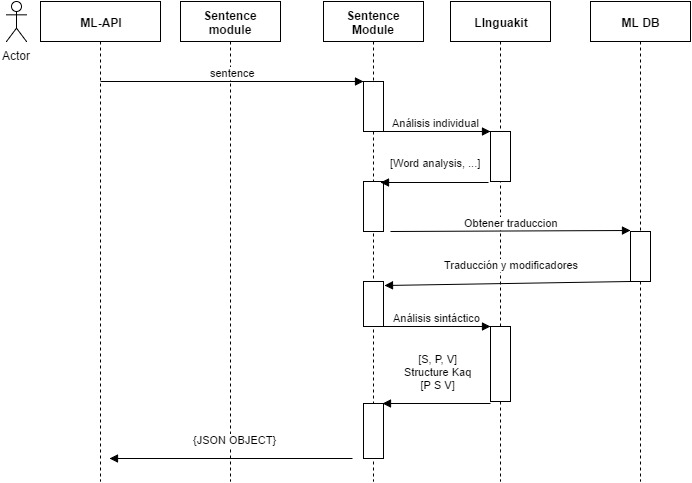
\includegraphics[width=1.1\textwidth]{secuenciaoracion}
	\caption{Diagrama de Secuencia de Oraciones}
	\label{fig:seco}
\end{figure}
Se presenta la secuencia que tiene una oración para ser traducida, muy parecido a la de una palabra, con la diferencia que Linguakit tiene una doble función, darnos el sentido de cada palabra y el sentido de toda la oración.

\subsection{Diagrama de Secuencia - Oraciones en otros Idiomas}
\begin{figure}[H]
	\centering
	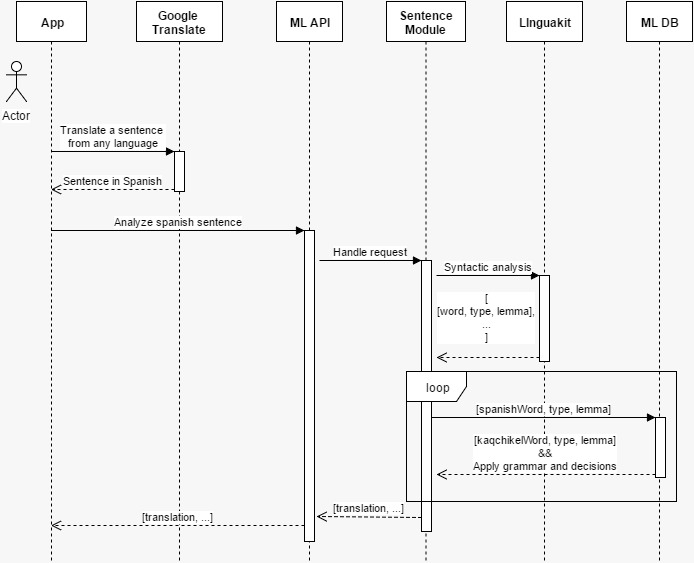
\includegraphics[width=1.2\textwidth]{secuenciaidiomas}
	\caption{Diagrama de secuencia de oración en otros idiomas}
	\label{fig:seci}
\end{figure}
Se presenta la secuencia que tiene una oración escrita en otro idioma para ser traducida. Se utiliza Google Translate para realizar esta traducción al español por lo que dicha oración puede ser escrita en cualquier idioma.

\newpage
\subsection{Diagrama de Casos de Uso}
\begin{figure}[h]
	\centering
	\includegraphics[width=0.8\textwidth]{casouso}
	\caption{Diagrama de Caso de Uso}
	\label{fig:caso}
\end{figure}
En este diagrama tenemos dos actores que tienen interacción MayaLeng. Contamos con el primer actor que es el usuario, el cual tiene la interacción de traducir palabras, traducir oraciones, y traducir cualquier palabra y oración de un idioma distinto al español, a kaqchikel.
\newpage

\subsection{Algoritmos implementados}
\subsubsection{Traducción de español a kaqchikel}
Lo que realiza este algoritmo, el cual es una implementación propia, se describe a continuación:

\begin{lstlisting}

Recibe texto
Si TextoMuyLargo Entonces
	Descomponer en oraciones mas cortas
	
Obtener palabras de oraciones
Mientras Palabras > 0
	Analizar tipo de palabra
	Si Palabra no tiene relacion gramatical Entonces
		Obtener traduccion de Palabra en kaqchikel
	Sino
		Analizar estructura gramatical en Kaqchikel
		Realizar traduccion de palabra
		Agregar funcion gramatical en Kaqchikel
		Devolver palabras traducidas
	
Analizar estructura de oracion en kaqchikel
Armar nueva oracion
Devolver nuevo texto

\end{lstlisting}
\newpage

\section{Conclusiones}
\begin{itemize}
	\item Aprendimos un poco más de la cultura de Guatemala, sobre las lenguas mayas.
	\item Pusimos en práctica varios temas de los aprendidos en la Universidad.
	\item Aprendimos nuevas tecnologías.
	\item Sobre todo luego de trabajar en este proyecto, siento que hemos aplicado nuestro conocimiento para ser útiles para la sociedad. Uno de los principales anhelos de cualquier persona, es ser útil.
	\item Aplicar nuestro conocimiento informático, hemos iniciado un proyecto que no termina acá, al contrario, hemos sentido también que con esto aportamos a la cultura y eso es satisfactorio.
	\item Hemos aprendido sobre el Kaqchikel, ya que antes de aplicar las reglas debimos haber entendido cómo hacerlo.
	\item Hemos experimentado con diversas tecnologías y con horas de desvelo, y no sólo porque esto nos sirva para ganar un curso, sino que creemos que esto puede de alguna manera cambiar nuestras vidas.
	\item Deseamos seguir trabajando en el proyecto, aplicar Inteligencia Artificial; en general hacer de esto un gran proyecto. Tenemos visión y las ganas de emprender esta aventura.
\end{itemize}
\newpage

\section{Recomendaciones}
\begin{itemize}
	\item Recomendamos aprender más sobre la cultura de Guatemala, no solamente de las lenguas mayas, que es de lo que trata este proyecto, sino en forma general, sobre historia, educación, logros, qué han hecho los guatemaltecos que han puesto el nombre de Guatemala en alto y saber que vivimos en un gran país con un gran potencial, y que podamos ser parte de ese crecimiento.
	\item En general el usuario exige una forma fácil de hacer las cosas, una forma interesante que le genere una necesidad de usar las cosas. Para próximas versiones es necesario entender el comportamiento del usuario contra las aplicaciones y mejorar esa experiencia. Evolucionar junto con las necesidades y exigencias del usuario promedio.
\end{itemize}
\newpage

\section{Referencias}
\begin{itemize}
	\item Filiberto Patal Majzul. (2007). Ruzoltzij Ri Kaqchikel. Guatemala|: Cholsamaj.
	\item (2006). Lenguas mayenses. 2006, de Wikipedia Sitio web: https://goo.gl/tpmgRJ
	\item (2002). Lenguas de Guatemala. 2002, de Wikipedia Sitio web: https://goo.gl/TRjvVQ
	\item Oracle Corporation. (2003). MySQL. 2016, de Wikipedia Sitio web: https://goo.gl/QhRXPt
	\item (1999). PHP 5 Introduction. 2016, de W3Schools Sitio web: https://goo.gl/lM91q
	\item (2002). Real Academia Española. 2016, de Wikipedia Sitio web: https://goo.gl/wU29ss
	\item (Año desconocido). Sobre Linguakit. 2016, de Linguakit Sitio web: https://goo.gl/LXE8gW
	\item What is Symfony., de Symfony Sitio web: https://goo.gl/GJmCR
	\item Perez J. J.. (2015). Qué es y cómo empezar con Ionic Framework. Noviembre 1, 2016, de PhoneGapSpain Sitio web: https://goo.gl/qOV5EP
	\item Google. Crea atractivos formularios., de Google Sitio web: https://goo.gl/XP1jpa
	\item (2002). LaTeX. 2016, de Wikipedia Sitio web: https://es.wikipedia.org/wiki/LaTeX
	\item WordPress Español. 2016, de WordPress Sitio web: https://goo.gl/DSb6kU
	\item Celso Lara Figueroa. (2014). Kaqchikel, Lengua de la Guatemala del maíz. 2016, de La Hora Sitio web: https://goo.gl/UNt5N5
\end{itemize}
\newpage

\section{Anexo}
\subsection{Calendarización}
\begin{figure}[h]
  \centering
    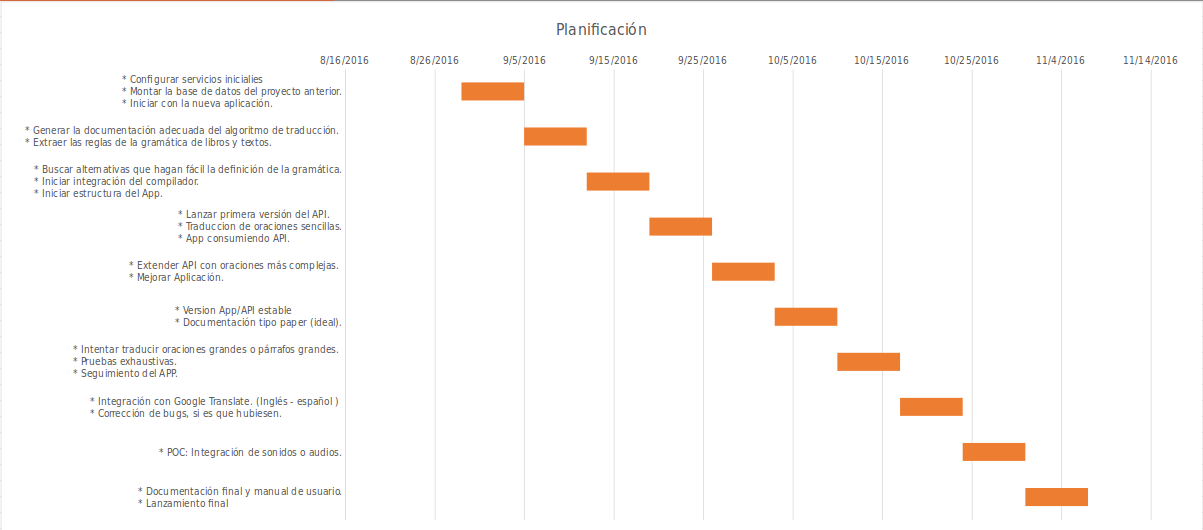
\includegraphics[width=1.0\textwidth]{Gantt}
  \caption{Diagrama de Gantt}
  \label{fig:gantt}
\end{figure}
Cronograma de trabajo inicial para el desarrollo del proyecto Mayaleng.

\subsection{Encuesta}
\begin{enumerate}
	\item ¿Le gustaría aprender una lengua maya?\\
	SI \rule{10mm}{0.1mm}  \hspace{5cm} NO \rule{10mm}{0.1mm}
	\item ¿Al visitar un departamento en Guatemala le gustaría poder comunicarse con personas que solamente conocen una lengua maya?	\\
	SI \rule{10mm}{0.1mm}  \hspace{5cm} NO \rule{10mm}{0.1mm}
	\item ¿Cree que aprender sobre la cultura de nuestro país es importante?\\
	SI \rule{10mm}{0.1mm}  \hspace{5cm} NO \rule{10mm}{0.1mm}
	\item ¿Usaría una aplicación móvil para aprender cosas básicas sobre lenguas mayas?\\
	SI \rule{10mm}{0.1mm}  \hspace{5cm} NO \rule{10mm}{0.1mm}
	\item ¿Pagaría por la aplicación?\\
	SI \rule{10mm}{0.1mm}  \hspace{5cm} NO \rule{10mm}{0.1mm}
	\item ¿Estaría dispuesto a invertir 10 minutos al día para conocer una lengua maya?\\
	SI \rule{10mm}{0.1mm}  \hspace{5cm} NO \rule{10mm}{0.1mm}
\end{enumerate}
Encuesta realizada a usuarios de los cuales todos contaban con un teléfono inteligente, la encuesta fue contestada por 79 personas.
\newpage

\section{Glosario}
\noindent 
\textbf{4G:} cuarta generación de tecnología de telefonía móvil.\\ \\
\textbf{Altruismo:} sacrificio personal en beneficio de otros. \\\\
\textbf{Android:} sistema operativo móvil de Google. \\\\
\textbf{AngularJS:} framework de JavaScript para crear y mantener aplicaciones web.\\ \\
\textbf{ANSI C:} estándar para el lenguaje de programación C para facilitar la portabilidad del código.\\ \\
\textbf{API:} utilizada por otro software como una capa de abstracción. \\\\
\textbf{C++:} lenguaje de programación.\\\\
\textbf{CLI:} interfaz de línea de comandos.\\ \\
\textbf{Cofradía:} Asociación de personas con unos mismos intereses, especialmente si estos son profesionales o altruistas.\\\\
\textbf{CRUD:} acrónimo de Crear, Leer, Actualizar y Borrar (Create, Read, Update and Delete).\\ \\
\textbf{CSS:} lenguaje de hojas de estilo para definición y presentación de sitios web.\\ \\
\textbf{DB:} base de datos. \\\\
\textbf{DBMS:} programa que permite almacenar y posteriormente acceder a los datos de forma rápida y estructurada.\\\\
\textbf{Enterprise:} versión de software empresarial.\\ \\
\textbf{Framework:} conjunto estandarizado de conceptos, prácticas y criterios para enfrentar y resolver nuevos problemas de índole similar. \\\\
\textbf{GNU:} sistema operativo de software libre.\\ \\
\textbf{GPL:} Licencia Pública General, la cual puede ser utilizada por cualquier persona o entidad.\\ \\
\textbf{HTML5:} versión 5 de HTML, lenguaje de marcado para elaboración de páginas web.\\ \\
\textbf{Ionic:} framework para desarrollo móvil.\\ \\
\textbf{iOS:} sistema operativo móvil de Apple. \\\\
\textbf{jQuery:} biblioteca de JavaScript que facilita interacción con HTML.\\ \\
\textbf{JS:} lenguaje de programación interpretado web JavaScript.\\ \\
\textbf{Kaqchikel:} lengua maya, parte de la familia lingüística mayense. \\\\
\textbf{LinguaKit:} programa para análisis del español. \\ \\
\textbf{LPPL:} licencia de software libre que no cumple con todos los requisitos de GPL.\\ \\
\textbf{MVC:} (Modelo Vista Controlador) patrón de arquitectura de software que separa los datos, la lógica y la interfaz de usuario.\\\\
\textbf{MySQL:}  sistema de gestión de bases de datos relacional. \\\\
\textbf{MySQL AB:} compañía de software creadora del DBMS MySQL.\\ \\
\textbf{Open source:} software cuyo código fuente es público.\\ \\
\textbf{PHP:} lenguaje de programación web. \\ \\
\textbf{Protomaya:} reconstrucción probable de la lengua origen de un grupo de lenguas.
\textbf{Responsive Web Design:} adaptar la apariencia de las páginas web al dispositivo que se esté utilizando para visualizarlas.  \\\\
\textbf{Sass:} (Syntactically Awesome Stylesheets), lenguaje de hojas de estilos traducido a CSS.\\ \\
\textbf{Script:} programa pequeño y simple almacenado en archivo de texto plano.\\ \\
\textbf{Symfony:} framework diseñado para optimizar el desarrollo de aplicaciones web.\\ \\
\textbf{Wordpress:} software para crear fácilmente sitios web.\\ \\
\newpage
\pagestyle{fancy}
\end{document}